\chapter{Teoría de la Computabilidad}\label{ch:teoria-de-la-computabilidad}
Clasificar los distintos problemas y formalizar el concepto de computar.

$\left\{\begin{matrix}
    Complejidad& \left\{\begin{matrix}
    Algoritmo &\rightarrow& \textit{Coste temporal } T(n)\\ 
    Problemas &\rightarrow& \textit{Tipo de problema según complejidad} \left\{\begin{matrix}
    P\\ 
    NP\\ 
    NPC
    \end{matrix}\right.
    \end{matrix}\right.\\ 
    Computabilidad& \rightarrow Problema \left\{\begin{matrix}
    Computable\\ 
    \textit{No computable}
    \end{matrix}\right.
    \end{matrix}\right.$

\textbf{Problema:} Descripción de una pregunta que requiere una respuesta.
\begin{itemize}
    \item p: instancia $\rightarrow$ respuesta
    \item $x \rightarrow p(x)$
\end{itemize}

\textbf{Instancia:} Especificación exacta de los datos de un problema para un caso particular.

\textbf{Algoritmo:} Conjunto de instrucciones que garantiza encontrar una solución correcta para cualquier instancia en un \textbf{número finito de pasos}.

\textbf{Analogía geométrica:} Hallar el lado de un cuadrado inscrito en un círculo, se puede dibujar fácilmente, pero en cuanto a matemáticas nunca se halla exactamente al tener raíces cuadradas. $r^2 = \frac{l^2}{2}+\frac{l^2}{2}; \; l= \sqrt{2}r$. Un caso en el que no es posible de ambas manera es dibujar un cuadrado con la misma área que un círculo, dado que entra en juego $\sqrt{\pi}$. $l^2 = \pi r^2; \; l = \sqrt{\pi}r$

\section{Problema de Satisfabilidad Booleana: SAT}
Un problema SAT2 puede ser...

if x then y else z

$(x \wedge y) \vee (\overline{x} \wedge z)$

\section{Clique}
Subgrafo completo, en el que todos los vértices están conectados con todos.

Tiene mucha potencia social, todos conocen o comparten gustos.

\section{Decidibilidad}
Un problema de computación puede considerarse como un lenguaje.

Las posibles soluciones del problema pueden considerarse como las palabras que pertenecen al lenguaje.
\begin{itemize}
    \item Ejem. $ax^2+bx+c=0$
    \item Problema: Tiene solución la ecuación en $\mathbb{R}$
    \item Respuestas $\in \{Si, No\}$
    \item Soluciones $\in \mathbb{R}$
    \item Lenguaje: $L= \{a,b,c\}$
\end{itemize}

\begin{figure}[H]
    \ffigbox[\FBwidth]
    {\caption{Diagrama Decidibilidad}}
    {\tikzset{every picture/.style={line width=0.75pt}}
    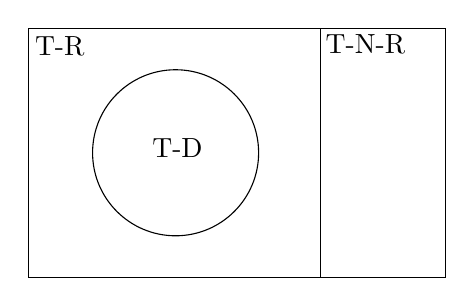
\begin{tikzpicture}[x=0.75pt,y=0.75pt,yscale=-1,xscale=1]
    \draw   (179,100) -- (380,100) -- (380,220) -- (179,220) -- cycle ;
    \draw   (210,160) .. controls (210,137.91) and (227.91,120) .. (250,120) .. controls (272.09,120) and (290,137.91) .. (290,160) .. controls (290,182.09) and (272.09,200) .. (250,200) .. controls (227.91,200) and (210,182.09) .. (210,160) -- cycle ;
    \draw    (320,100) -- (320,220) ;
    
    \draw (181,103) node [anchor=north west][inner sep=0.75pt]   [align=left] {T-R};
    \draw (321,102) node [anchor=north west][inner sep=0.75pt]   [align=left] {T-N-R};
    \draw (237.5,152) node [anchor=north west][inner sep=0.75pt]   [align=left] {T-D};
    \end{tikzpicture}}
\end{figure}
\begin{itemize}
    \item \textbf{T-D:} Turing-Decidible. Es un problema para el cual una MT acepta todas las soluciones y rechaza las que no son. \\ Se para siempre.
    \item \textbf{T-R:} Turing-Reconocible, pero no decidible. Es un problema para el cual la MT acepta todas las que son soluciones. \\ Puede entrar en bucle para las no soluciones.
    \item \textbf{T-N-R:} Turing-No-Reconocible. Ni acepta las que son soluciones, ni rechaza las que no son. \\ Entra en bucle.
\end{itemize}

Un T-D es un T-R, siguiendo el diagrama

\textbf{Reconocer} un problema (lenguaje) es aceptar todas las soluciones del problema.

\textbf{Decidir} un problema es:
\begin{itemize}
    \item Reconocer todas las soluciones.
    \item Rechazar todas las no-soluciones.
\end{itemize}

Solo los T-D se llaman Computables o Decidibles.
\begin{itemize}
    \item Ejem. El teorema de Fermat ($x^n + y^n = z^n$ con $n>2 / n \in \mathbb{R}$) es indecible porque ni computacional ni matemáticamente no se puede demostrar, aunque se sabe que no hay otro real que cumpla la condición aparte de 2. La máquina estaría infinitamente probando valores.
\end{itemize}

CUIDADO. Indecidible no especifica si es T-R o T-N-R, a veces al T-R se le llama parcialmente decidible.

\textbf{MT Reconocedora:} Que no genera salida lee la cinta, pero no lo modifica/manipula.

\textbf{MT Transductora:} Que genera salida. Modifica la cinta, además de reconocer la cinta.